% ============================================================
%   main.tex —— Lab Report (Main File)
% ============================================================

\documentclass[12pt, a4paper]{article}
\usepackage{report-style}


\begin{document}

% ============================================================
%   Page 1: Cover Page
% ============================================================
\newgeometry{top=3cm, bottom=3cm, left=3.5cm, right=2.5cm}

\begin{center}
    \vspace*{0.5cm}
    {\fontsize{26pt}{30pt}\selectfont\bfseries xxxx\enspace xxxx\enspace xxxx\enspace xxxx\enspace 实\enspace 验\enspace 报\enspace 告}
    \vspace{2cm}
\end{center}

\newcommand{\mline}[2]{%
    \noindent\mbox{\zihao{4}\bfseries #1：\underline{\makebox[10cm][l]{#2}}}\\[3ex]%
}

\vspace{0.5cm}
\begin{flushleft}
    \mline{课程名称}{xxxx}
    \mline{实验项目名称}{xxxx}
    \mline{学\hspace{2em}院}{xxxx学院}
    \mline{专\hspace{2em}业}{xxxx}
    \mline{指导教师}{xxxx}
    \noindent\mbox{\zihao{4}\bfseries
        报告人：\underline{\makebox[3cm][l]{xxxx}}%
        \hspace{1.5em}学号：\underline{\makebox[3.5cm][l]{xxxx}}%
        \hspace{1.5em}班级：\underline{\makebox[3cm][l]{xxxx}}%
    }\\[3ex]
    \mline{实验时间}{xxxx 年 xx 月 xx 日}
    \mline{实验报告提交时间}{xxxx 年 xx 月 xx 日}
\end{flushleft}

\vfill
\begin{center}
    {\large \textbf{教\enspace 务\enspace 部\enspace 制}}
\end{center}

\newpage
\restoregeometry


% ============================================================
%   I. Objectives and Requirements
% ============================================================
\begin{labbox}{一、实验目的与要求：}{}

\begin{itemize}[leftmargin=2em, itemsep=0.3em]
    \item xxxx
    \item xxxx
    \item xxxx
    \item xxxx
    \item xxxx
\end{itemize}

\end{labbox}


% ============================================================
%   II. Methodology and Procedures
% ============================================================
\begin{labbox}{二、实验方法与步骤：}{}

\begin{enumerate}[leftmargin=2em, itemsep=0.5em]

    \item \textbf{xxxx}

    打开 xxxx，依次执行：
\begin{lstlisting}
xxxxxxxxxxxxxxxxxxxx
xxxxxxxxxxxxxxxxxxxx
\end{lstlisting}

    \item \textbf{xxxx}
\begin{lstlisting}
xxxxxxxxxxxxxxxxxxxx
\end{lstlisting}

    安装完成后验证：
\begin{lstlisting}
xxxxxxxxxxxxxxxxxxxx
\end{lstlisting}

    \item \textbf{xxxx}

    xxxx 步骤如下：
\begin{center}
    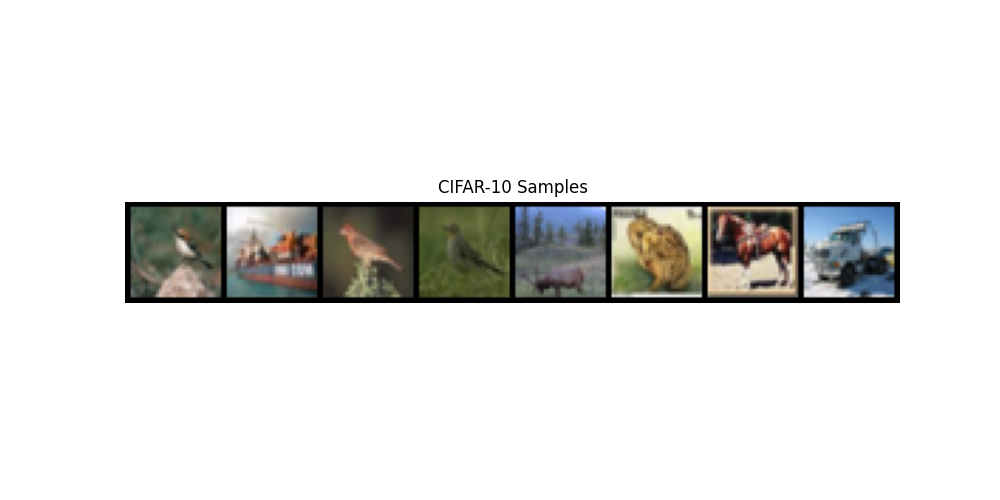
\includegraphics[width=0.8\linewidth]{xxxx.png}
    \par\vspace{0.2em}
    {\small 图1\quad xxxx}
\end{center}
\begin{center}
    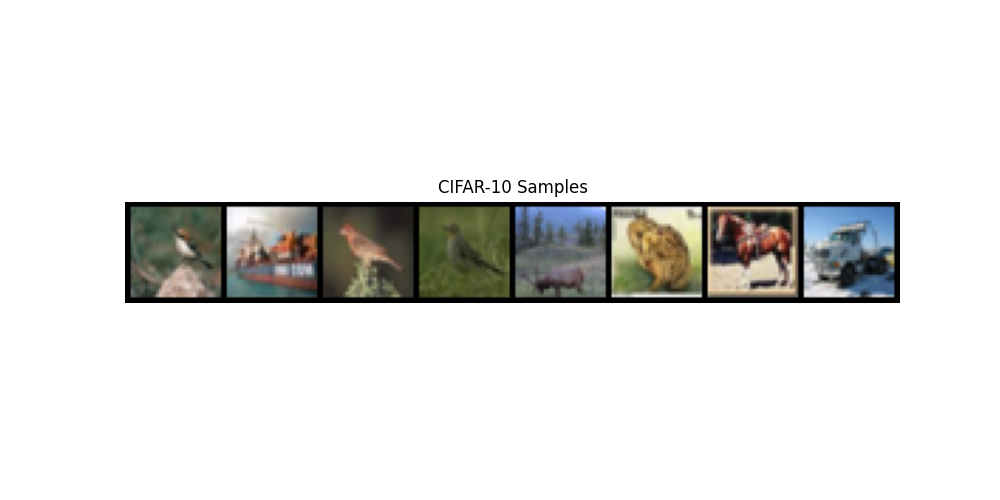
\includegraphics[width=0.8\linewidth]{xxxx.png}
    \par\vspace{0.2em}
    {\small 图2\quad xxxx}
\end{center}
\begin{center}
    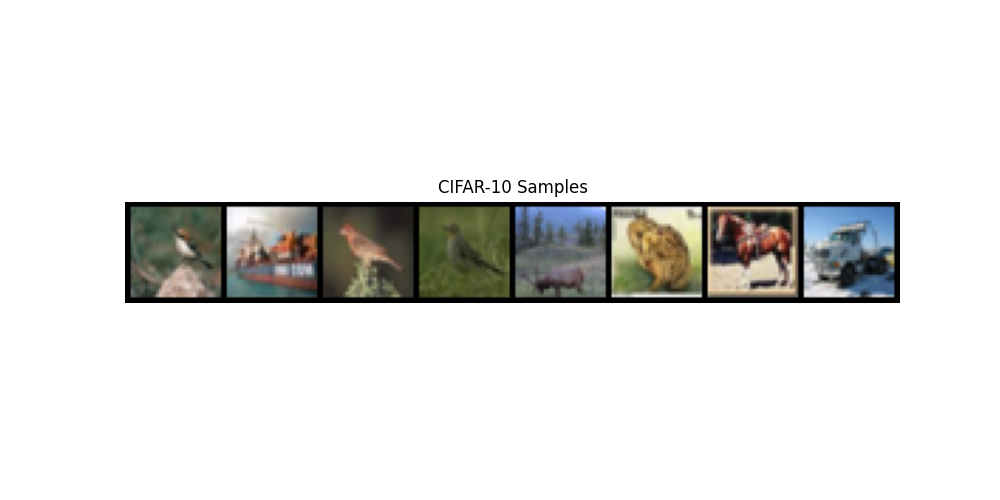
\includegraphics[width=0.8\linewidth]{xxxx.png}
    \par\vspace{0.2em}
    {\small 图3\quad xxxx}
\end{center}

    \begin{enumerate}[label=\alph*., leftmargin=2em, itemsep=0.2em]
        \item xxxx \url{xxxx}，xxxx。
        \item xxxx \textbf{xxxx}，xxxx。
        \item xxxx \textbf{xxxx}，xxxx。
        \item xxxx：
\begin{lstlisting}
xxxxxxxxxxxxxxxxxxxx
\end{lstlisting}
        \item xxxx \texttt{xxxx}，xxxx。
    \end{enumerate}
\begin{center}
    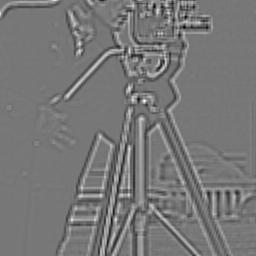
\includegraphics[width=0.8\linewidth]{xxxx.jpg}
    \par\vspace{0.2em}
    {\small 图4\quad xxxx}
\end{center}
    \item \textbf{xxxx}

    xxxx：
\begin{lstlisting}
xxxx/
  xxxx/
    xxxx/
    xxxx/
  xxxx/
    xxxx/
    xxxx/
  xxxx
\end{lstlisting}

    \item \textbf{xxxx}

    新建 \texttt{xxxx}，内容见第三节，然后运行：
\begin{lstlisting}
xxxxxxxxxxxxxxxxxxxx
\end{lstlisting}

    \textbf{注意：} xxxx。

    \item \textbf{xxxx}

    训练完成后运行：
\begin{lstlisting}
xxxxxxxxxxxxxxxxxxxx
\end{lstlisting}

    xxxx。

\end{enumerate}

\end{labbox}

% ============================================================
%   III. Experimental Process and Content
% ============================================================
\begin{labbox}{三、实验过程及内容：}{}

\textbf{（1）训练脚本 \texttt{xxxx}}

\begin{lstlisting}
xxxxxxxxxxxxxxxxxxxx
xxxxxxxxxxxxxxxxxxxx
xxxxxxxxxxxxxxxxxxxx
xxxxxxxxxxxxxxxxxxxx
xxxxxxxxxxxxxxxxxxxx
xxxxxxxxxxxxxxxxxxxx
xxxxxxxxxxxxxxxxxxxx
xxxxxxxxxxxxxxxxxxxx
\end{lstlisting}

\textbf{（2）推理脚本 \texttt{xxxx}}

\begin{lstlisting}
xxxxxxxxxxxxxxxxxxxx
xxxxxxxxxxxxxxxxxxxx
xxxxxxxxxxxxxxxxxxxx
xxxxxxxxxxxxxxxxxxxx
xxxxxxxxxxxxxxxxxxxx
xxxxxxxxxxxxxxxxxxxx
\end{lstlisting}

\textbf{（3）xxxx 简介}

xxxx：
\begin{itemize}[leftmargin=2em, itemsep=0.2em]
    \item \textbf{xxxx}：xxxx。
    \item \textbf{xxxx}：xxxx。
    \item \textbf{xxxx}：xxxx。
\end{itemize}

\vspace{0.3cm}
\textbf{（4）Inserting Screenshots and Descriptions}

% Single Image
\begin{center}
    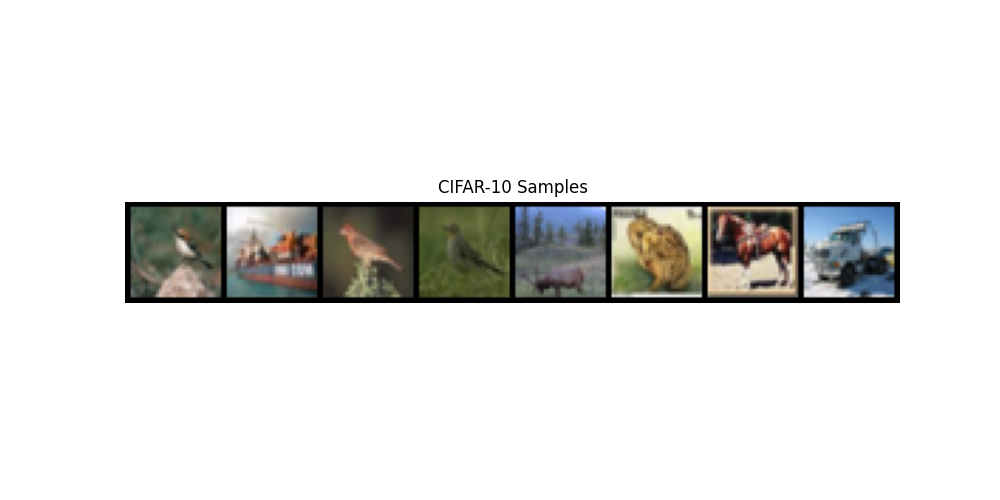
\includegraphics[width=0.8\linewidth]{xxxx.png}
    \par\vspace{0.2em}
    {\small 图1\quad xxxx}
\end{center}

% Two images side by side
% \begin{center}
%     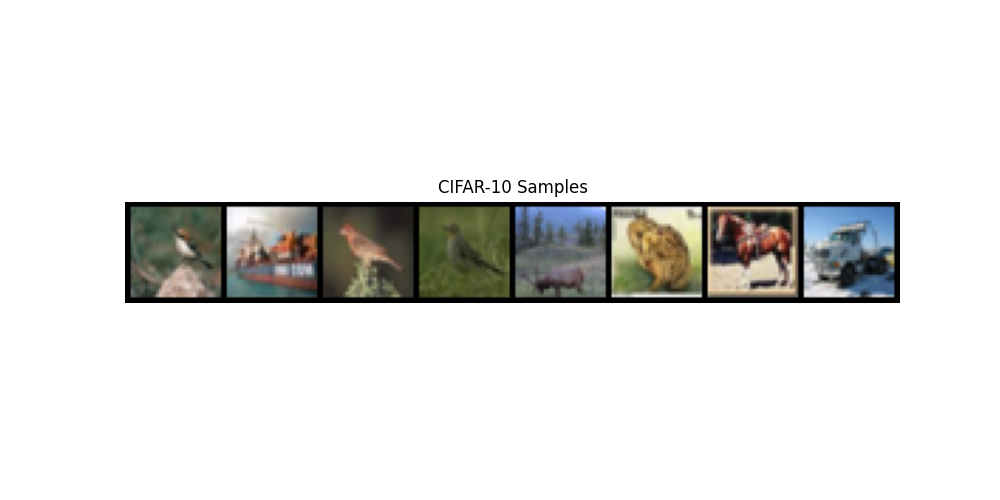
\includegraphics[width=0.48\linewidth]{xxxx.png}
%     \hfill
%     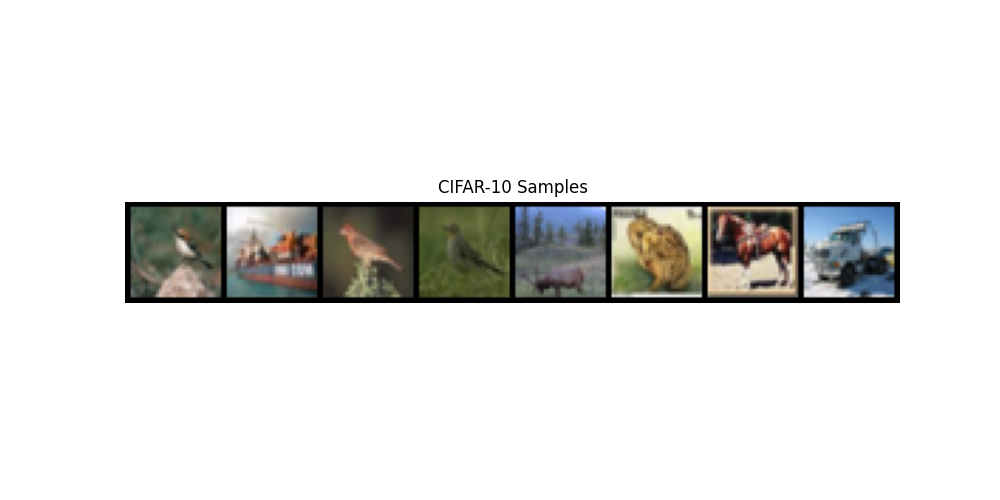
\includegraphics[width=0.48\linewidth]{xxxx.png}
%     \par\vspace{0.2em}
%     {\small 图2\quad xxxx}
% \end{center}

\end{labbox}


% ============================================================
%   IV. Data Processing and Analysis
% ============================================================
\begin{labbox}{四、数据处理与分析：}{}

xxxx：

\vspace{0.3cm}
\begin{center}
\begin{tabular}{|c|c|c|c|c|}
    \hline
    \textbf{xxxx} & \textbf{xxxx} & \textbf{xxxx} & \textbf{xxxx} & \textbf{xxxx} \\
    \hline
    x & x & x & x & x \\
    x & x & x & x & x \\
    x & x & x & x & x \\
    x & x & x & x & x \\
    \hline
\end{tabular}
\end{center}
\vspace{0.3cm}

\textbf{Metric Definitions:}
\begin{itemize}[leftmargin=2em, itemsep=0.2em]
    \item \textbf{xxxx}：xxxx。
    \item \textbf{xxxx}：xxxx。
    \item \textbf{xxxx}：xxxx。
    \item \textbf{xxxx}：xxxx。
\end{itemize}

\vspace{0.2cm}
xxxx（xxxx）。

\end{labbox}


% ============================================================
%   V. Conclusion
% ============================================================
\newpage
\begin{labbox}{五、实验结论：}{}

\begin{enumerate}[leftmargin=2em, itemsep=0.4em]
    \item xxxx
    \item xxxx
    \item xxxx
    \item xxxx
    \item xxxx
\end{enumerate}

\end{labbox}

% ---------- Instructor Review Section ----------
\begin{labbox}{}{9cm}
    \hspace{1em}\zihao{-4}指导教师批阅意见：\\[3.5cm]
    \hspace{1em}成绩评定：\\[2cm]
    \hfill 指导教师签字：\hspace{4em} \\
    \hfill \makebox[3em]{}年\makebox[2em]{}月\makebox[2em]{}日\hspace{2em} \\[0.5em]
\end{labbox}

% ---------- Remarks ----------
\begin{labbox}{备注：}{}
    无
\end{labbox}

% ---------- Footer Notes ----------
\begin{spacing}{1.2}
    \zihao{5}
    \noindent 注：\begin{minipage}[t]{0.88\textwidth}
        1、xxxx。\\
        2、xxxx。
    \end{minipage}
\end{spacing}

\end{document}